%\documentclass[varwidth]{standalone}
\documentclass[10pt]{amsart}
\usepackage{amscd,amsxtra,color,amsthm}

\usepackage[all]{xy}
\usepackage{etex}
\usepackage{pictex}
\usepackage{graphicx}
\usepackage{tikz}
\usepackage[utf8]{inputenc} 
\usepackage[T1]{fontenc}
\usepackage[all]{xy}
\usepackage{etex}
\usepackage{pictex}
\usepackage{graphicx}
\usepackage{mathtools}
\DeclarePairedDelimiter{\ceil}{\lceil}{\rceil}
\DeclarePairedDelimiter{\floor}{\lfloor}{\rfloor}
\usepackage{comment}
\usepackage{changepage}


\textheight=9in \textwidth=6.2in \topmargin=0in
\oddsidemargin=.15in \evensidemargin=.15in

\begin{document}
\parskip10pt
\parindent12pt
\baselineskip16pt





%%%%%%%%%%%%%%%%%%%%%%%%%%%%%%%%%%%%%%%%%%%%%%%%%%%%%%%%%%%%%%%%%%%%%%%%%%%%%%%%%%%%%%%%%%%%%%%%
%%  Definitions
%%%%%%%%%%%%%%%%%%%%%%%%%%%%%%%%%%%%%%%%%%%%%%%%%%%%%%%%%%%%%%%%%%%%%%%%%%%%%%%%%%%%%%%%%%%%%%%%

\def\G{\widetilde{G}}
\def\B{\widetilde{B}}
\def\T{\widetilde{T}}
\def\C{\mathbb{C}}
\def\A{\mathbb{A}}
\def\Z{\mathbb{Z}}
\def\R{\mathbb{R}}
\def\Q{\mathbb{Q}}
\def\N{\mathbb{N}}
\def\C{\mathbb{C}}
\def\F{\mathbb{F}}
\def\I{\mathbb{I}}
\def\H{\mathcal{H}}
\def\e{\varepsilon}
\def\s{\underline s}
\def\z{\zeta }
\def\vp{\varpi }
\def\O{\mathcal O}
\def\v{\upsilon }
\def\U{\Upsilon }
\def\p{\wp }
\def\p{\mathfrak{p}}
\def\B{\mathfrak{B}}

\newtheorem{theorem}{Theorem}%[section]
\newtheorem{lemma}[theorem]{Lemma}


\title{Proof for Closed Eulerian Trails}

\author{Graham Swain}
%\centerline{Your name goes here.}




\begin{abstract}
In this paper we explore a proof showing that a graph contains a closed Eulerian trail if and only if
all of its vertices have even degree. We show this with a direct proof and by developing an algorithm.
\end{abstract}

\maketitle



%\begin{abstract}
%abstract goes here....
%\end{abstract}

%\maketitle

\section{Introduction}

This problem dates back to 18th century K\"{o}nigsberg, Prussia, modern day Kaliningrad, Russia. 
K\"{o}nigsberg had seven bridges that connected four landmasses, the figure below shows roughly 
how the bridges were arranged. The citizens of K\"{o}nigsberg wonder if a person could walk across 
town and cross each bridge exactly once.

\begin{figure}[h!]
\centerline{
{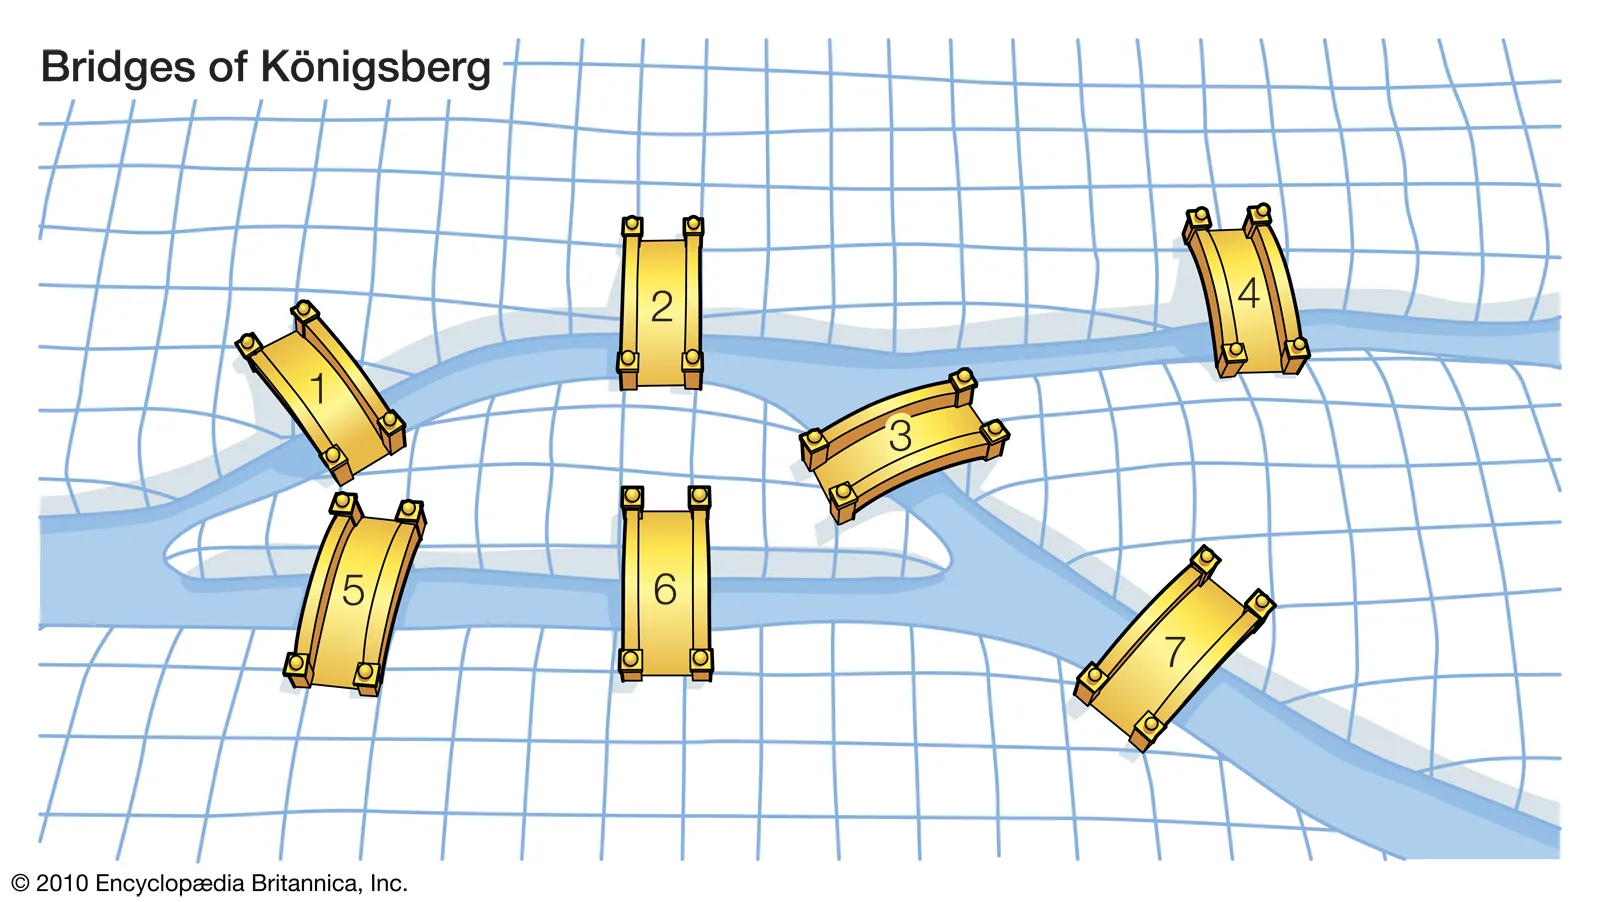
\includegraphics[width=.7\textwidth]{pictures/bridge_pic.png}}}\label{bridge}
\end{figure} 

The problem was solved by Leonard Euler, who found it to be impossible. His reasoning was that 
every time you enter a landmass you must also be able to leave it, so any landmass with an odd
number of bridges coming from it would cause you to get stuck. There is an exception for the landmass
that you start and as well as the one you end on, but in K\"{o}nigsberg each landmass has an odd 
number of bridges coming from them. This led to the theorem we are looking at today as well as 
set the basis for modern day graph theory.

\section{Definitions}
\noindent
Before we look at the theorem, we first must go over some definitions to help understand it.

\noindent
\textbf{Definition} 
\emph{
    A \textbf{graph} G = (V,E) is comprised of a set of vertices V and a set of 
    different unordered pairs of distinct vertices from V called E. Elements from E are called edges.
}

\noindent
\textbf{Definition} 
\emph{
    Two vertices v, w that exist in V are said to be \textbf{adjacent} if the
    edge vw exists in E.
}

\noindent
\textbf{Definition}
\emph{
    If ab exists in E, then we say that the vertex v and the edge vw are \textbf{incident}; w would
    also be incident with vw.
}

\noindent
\textbf{Definition}
\emph{
    The \textbf{degree} of a vertex v that exists in V is the amount of edges in E that are incident
    with v.
}

\noindent
\textbf{Definition}
\emph{
    A \textbf{walk} W is a finite sequence of vertices in which each consecutive pair of vertices
    are adjacent.
}
Vertices and edges are allowed to be repeated in a walk, with the exception of the same vertex consecutively,
to prevent loops.

\noindent
\textbf{Definition}
\emph{
    A \textbf{trail} T is a walk in which edges are not allowed to be repeated. A trail is called a 
    \textbf{closed trail} when the trail begins and ends at the same vertex.
}

\noindent
\textbf{Definition}
\emph{
    A trail that contains all of the edges in E is called an \textbf{Eulerian trail}. A \textbf{closed
    Eulerian trail} when the trail begins and ends at the same vertex.
}

\noindent
\textbf{Definition}
\emph{
    A graph is said to be \textbf{connected} if, and only if, there is a walk between any two vertices
    v and w.
}

\section{Theorem and Proof}

\begin{theorem} \ 
    A connected graph has a closed Eulerian trail if and only if all of its vertices have even degree.
    \label{theorem1}
\end{theorem}

\begin{proof} 
    ($\Rightarrow$) Assume a connected graph $G$ has a closed Eulerian trail, denoted as $C$. Prove that
    every vertex has an even degree. 
    
    \noindent
    Take an arbitrary vertex $v$. As we traverse $C$, each time we enter $v$ we must be able to exit on a
    distinct edge. Thus every vertex must be incident with 2$k$ edges, where $k$ is the number of times
    a vertex is visited. Therefore every vertex has an even degree. 

    \noindent
    The first vertex of $C$ does make a special case. It does not matter since we chose an arbitrary
    vertex in the first step, but we can still look at it. Denote the first vertex of $C$ as $a$. We
    know that $a$ is incident to the first edge of $C$, the last edge of $C$, as well as a 2$k$ amount
    of other edges. So $a$ is adjacent to \\
    \centerline{$1+2k+1 = 2+2k$} \\
    edges, which will result in an even number.

    \noindent
    ($\Leftarrow$) Assume $G$ is a connected graph with every vertex having even degree. Prove that
    it has a closed Eulerian trail.

    \begin{figure}[h!]
        \centerline{
        {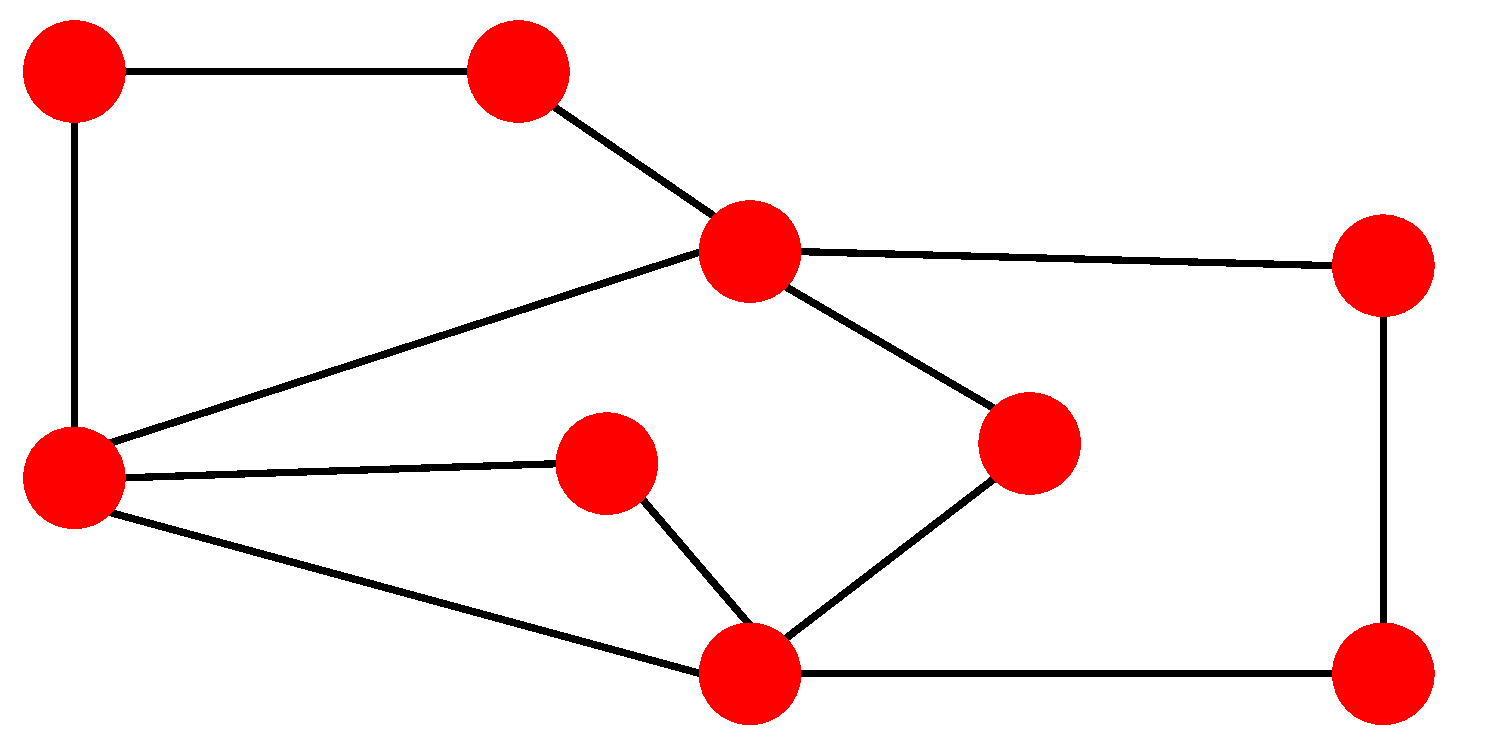
\includegraphics[width=.45\textwidth]{pictures/G.pdf}}}
        \caption{Graph $G$ we will look at as we construct the algorithm.}\label{G}
    \end{figure} 

    \noindent
    To prove this direction we must construct an algorithm. 
    
    \noindent
    \textbf{Step 1.} Pick an arbitrary vertex $v$ to act as our starting point.

    \noindent
    \textbf{Step 2.} Construct a trail beginning at $v$. Continue to add edges to this trail until we
    arrive back at $v$. (\emph{We know we arrived at $v$ since if we entered another vertex $a$ that we
    could not leave then $a$ has an edge to enter on but not a corresponding edge to exit on. Which would
    mean that $a$ has an odd degree, which would be a contradiction.}) Since we did arrive back at
    $v$ we formed a closed trail, which we will called $C_1$.

    \begin{figure}[h!]
        \centerline{
        {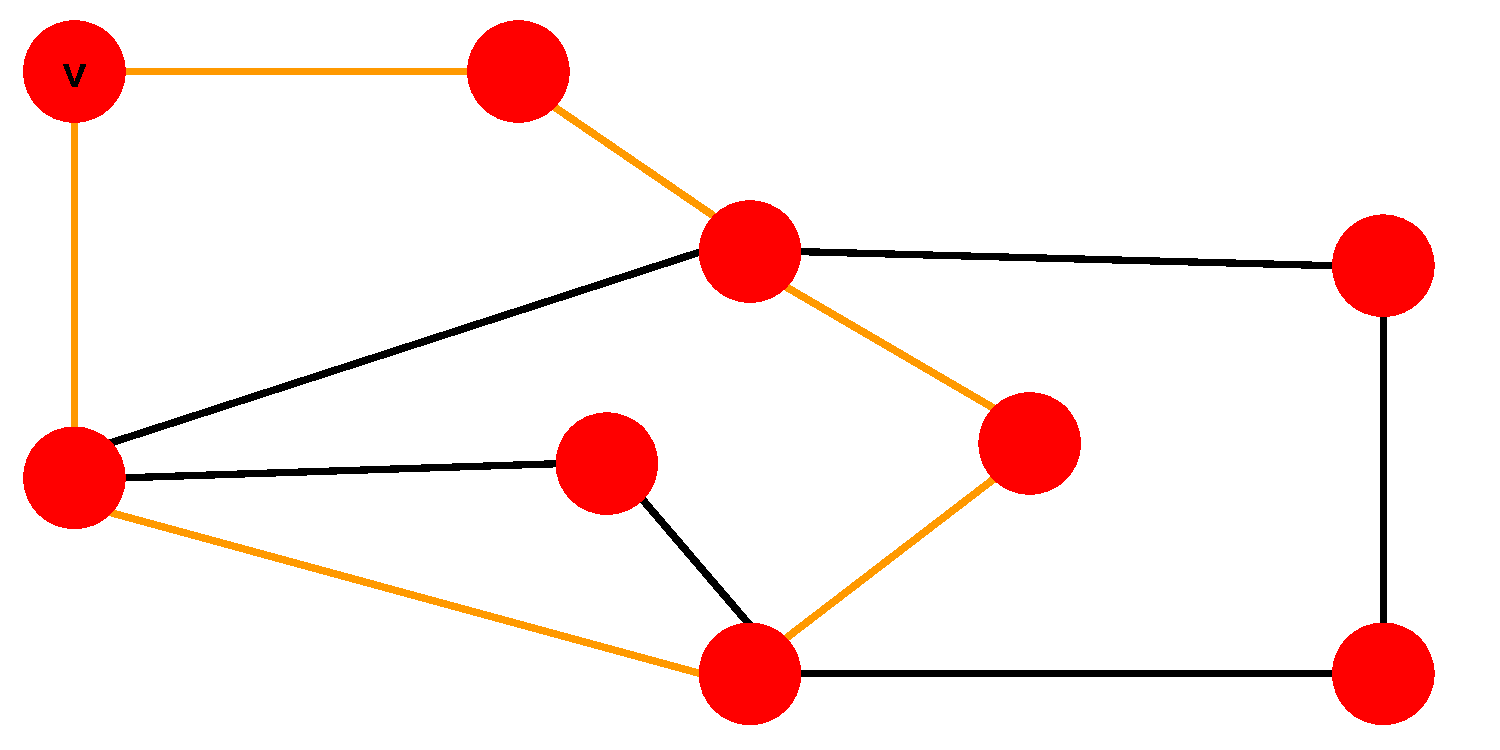
\includegraphics[width=.45\textwidth]{pictures/C1.pdf}}}
        \caption{$C_1$ is highlighted in orange.}\label{C1}
    \end{figure} 

    \noindent
    \textbf{Step 3.} Check if $C_1$ contains all the edges of $G$. If it does we have found a closed
    Eulerian trail and are done. If it does not contain all of the edges of $G$ then we continue to
    \textbf{Step 4}.

    \noindent
    \textbf{Step 4.} Remove all of the edges in $C_1$ from $G$. We will call the resulting graph $G'$.
    ($G'$ does not need to be connected).

    \begin{figure}[h!]
        \centerline{
        {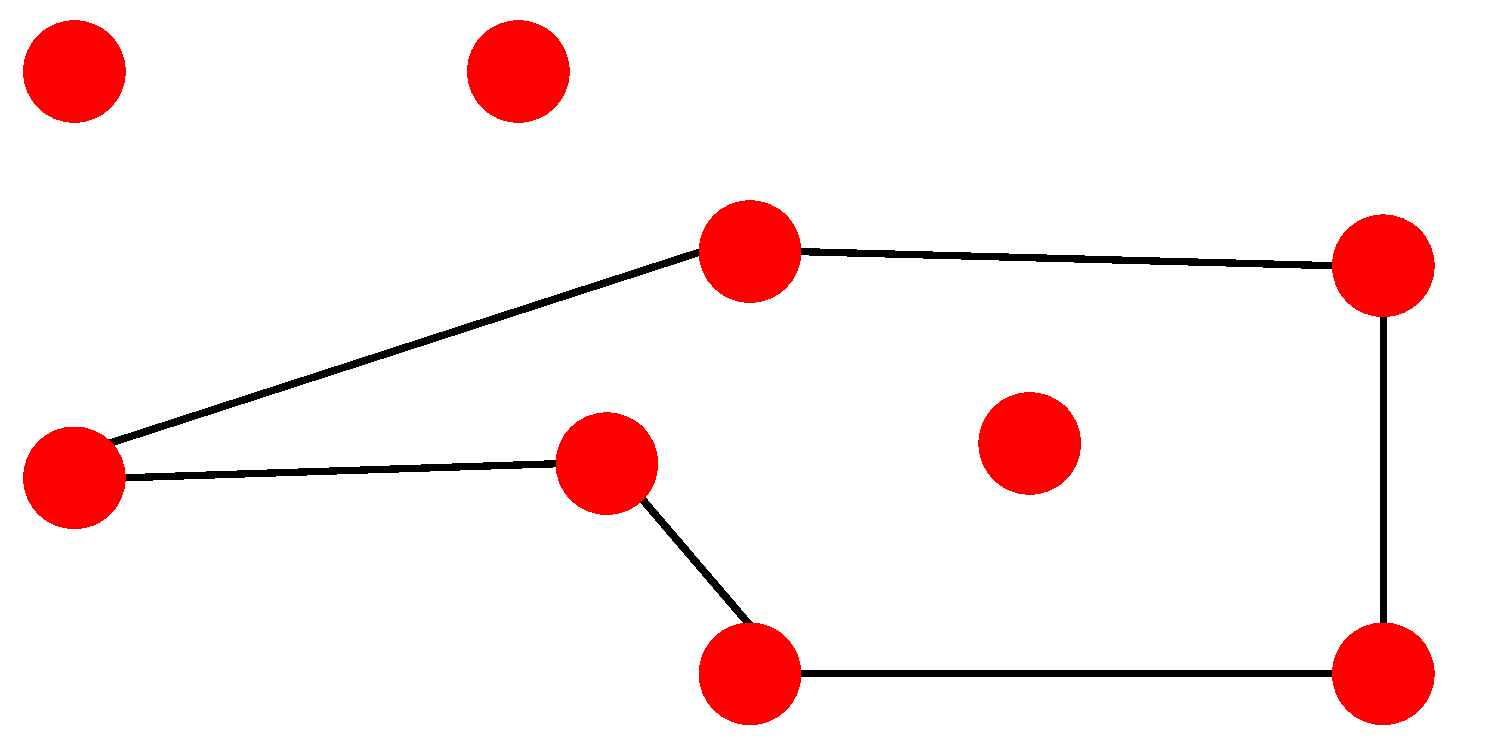
\includegraphics[width=.45\textwidth]{pictures/G'.pdf}}}
        \caption{The remaining edges after we remove $C_1$ from $G$ form $G'$.}\label{G2}
    \end{figure} 

    \noindent
    \textbf{Step 5.} Choose an arbitrary vertex $w$ that is in both $C_1$ and $G$.

    \noindent
    \textbf{Step 6.} Construct a trail in $G'$ beginning at $w$ and continue until we arrive back at
    $w$. We will call the resulting closed trail $C_2$.

    \begin{figure}[h!]
        \centerline{
        {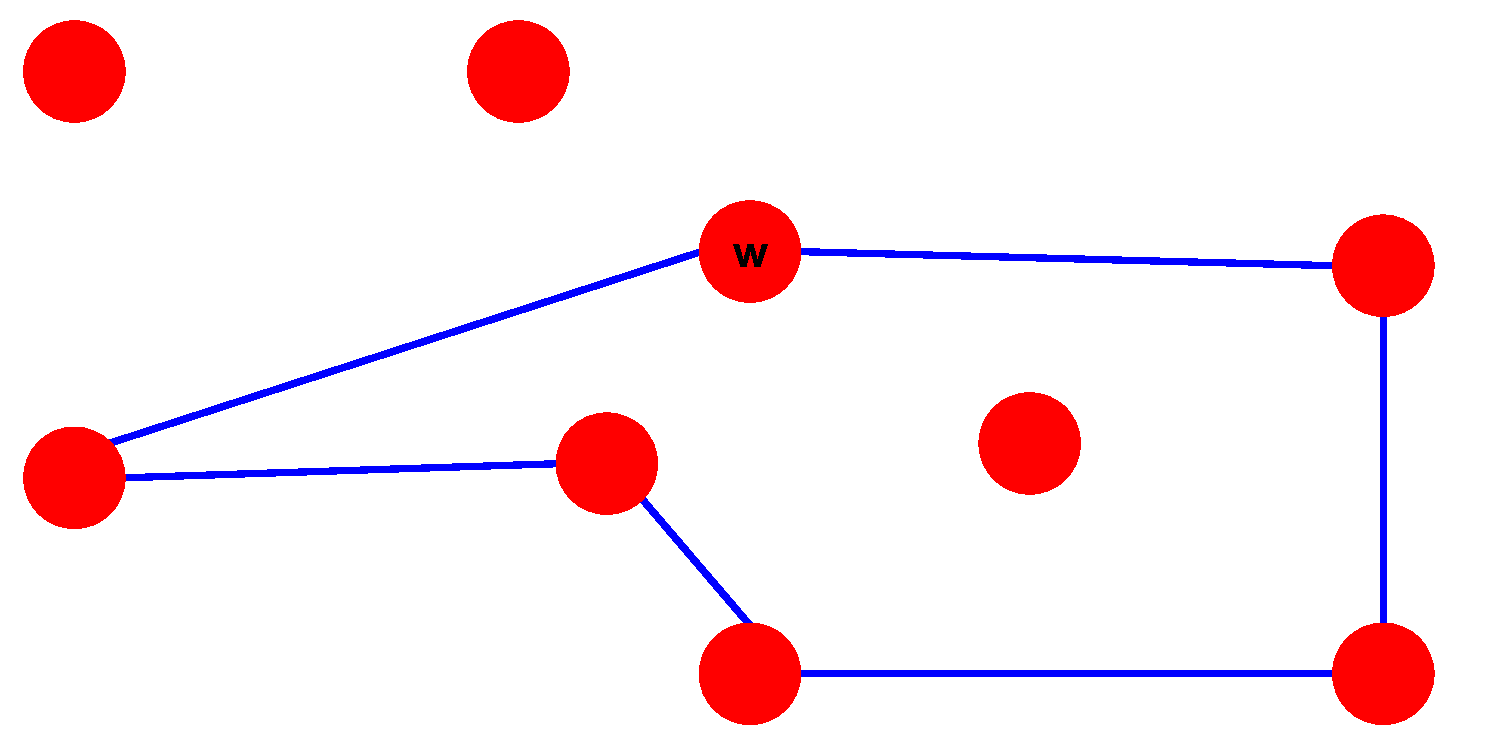
\includegraphics[width=.5\textwidth]{pictures/C2.pdf}}}
        \caption{$C_2$ is highlighted in blue.}\label{C2}
    \end{figure} 

    \noindent
    \textbf{Step 7.} Combine $C_1$ and $C_2$ to form a new closed trail denoted as $C'$. If $C'$
    contains all of the edges of $G$, we have found a closed Eulerian trail and are done. If not 
    continue to \textbf{Step 8.}

    \begin{figure}[h!]
        \centerline{
        {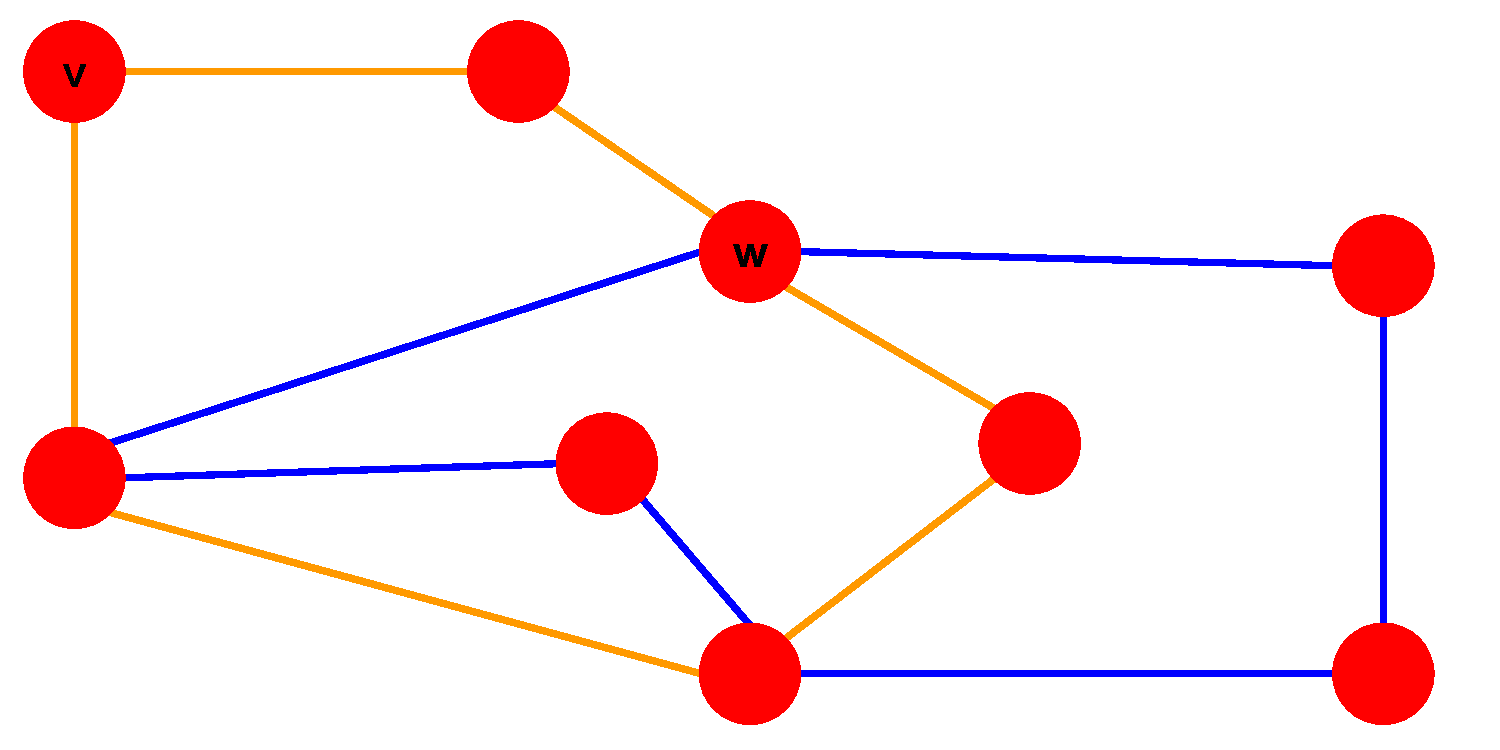
\includegraphics[width=.5\textwidth]{pictures/C'.pdf}}}
        \caption{$C'$ is formed by combining $C_1$ and $C_2$. $C'$ does contain all of the edges of
        $G$, so we are done in this example.}\label{C'}
    \end{figure} 

    \noindent \emph{
        We know that combining two closed trails form a new closed trail. To show this, start at $v$
        in $C_1$. Trace $C_1$ until we arrive at $w$. Once we reach $w$, trace the entirety of $C_2$.
        Once we arrive back at $w$, continue tracing $C_1$ until we end at $v$. The trace is $C'$.
    }

    \begin{figure}[h!]
        \centerline{
        {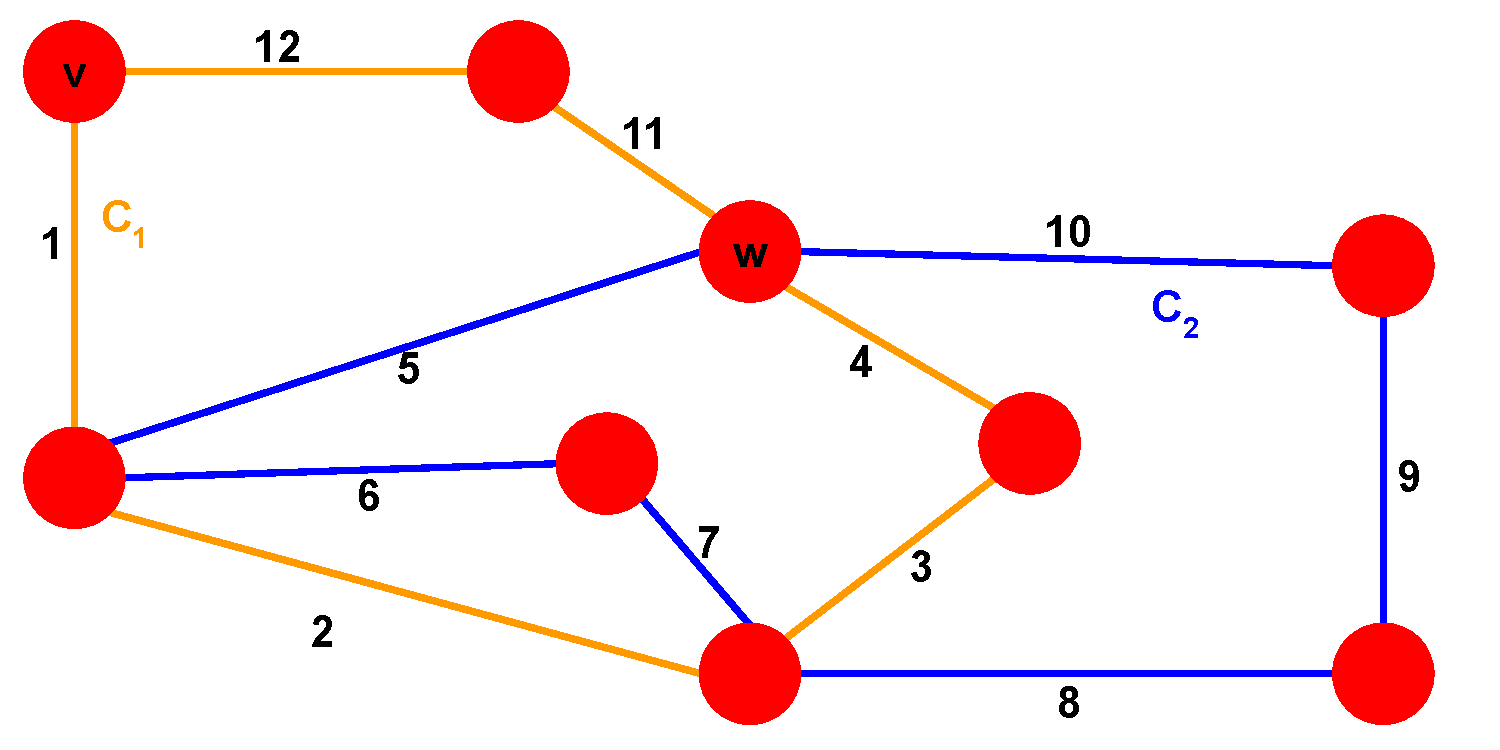
\includegraphics[width=.5\textwidth]{pictures/c'_traversal.pdf}}}
        \caption{Followed the number trail to see how two closed trails can be combined to formed
        another closed trail.}\label{C_traverse}
    \end{figure} 

    \noindent
    \textbf{Step 8.} Remove all of the edges of $C'$ from $G$ to get $G''$. Chose a vertex in both
    $C'$ and $G''$ and continue in this manner until we have removed all the edges of $G$.

    \noindent    
\end{proof}

This theorem is highly related to another theorem dealing with Eulerian trails.

\begin{theorem} \label{theorem2}
    A connected graph has an Eulerian trail but not an closed Eulerian trail if and only if it has
    exactly two vertices of odd degree.
\end{theorem}


We will not make a formal proof of this theorem, but we can look at it intuitively. The difference
between an Eulerian trail and closed Eulerian trail is that a closed Eulerian trail begins and ends
at the same vertex. So to have an Eulerian trail that is not closed we know that the first vertex $a$
must be distinct from the last vertex $z$. In the proof of Theorem \ref{theorem1} we found that the
beginning vertex must be incident to $2k+2$ edges, since the first edge and the last edge are both
incident to it. So it follows that $a$ and $z$ would be incident to $2k+1$ edges, since $a$ is incident
to the first edge but not the last and the opposite is true for $z$. All of the other edges would still
be incident to $2k$ edges. For the other direction we can prove using the same algorithm. The only
difference is we need to make a new "fake" edge between $a$ and $z$ to temporarily form a closed
Eulerian trail. Once we are done with the algorithm we can remove $az$ to return to a Eulerian trail
that is not closed.

\section{Conclusion}

It should now be clear why it was impossible to take a trip across K\"{o}nigsberg and cross each bridge
exactly once. Figure \ref{g_bridge} shows the bridges as a graph, with the landmass as the vertices and the 
bridges as the edges. You can see how the vertex on the left has a degree of five and that the others
have degree three, so there is no closed Eulerian trail.

\begin{figure}[h!]
    \centerline{
    {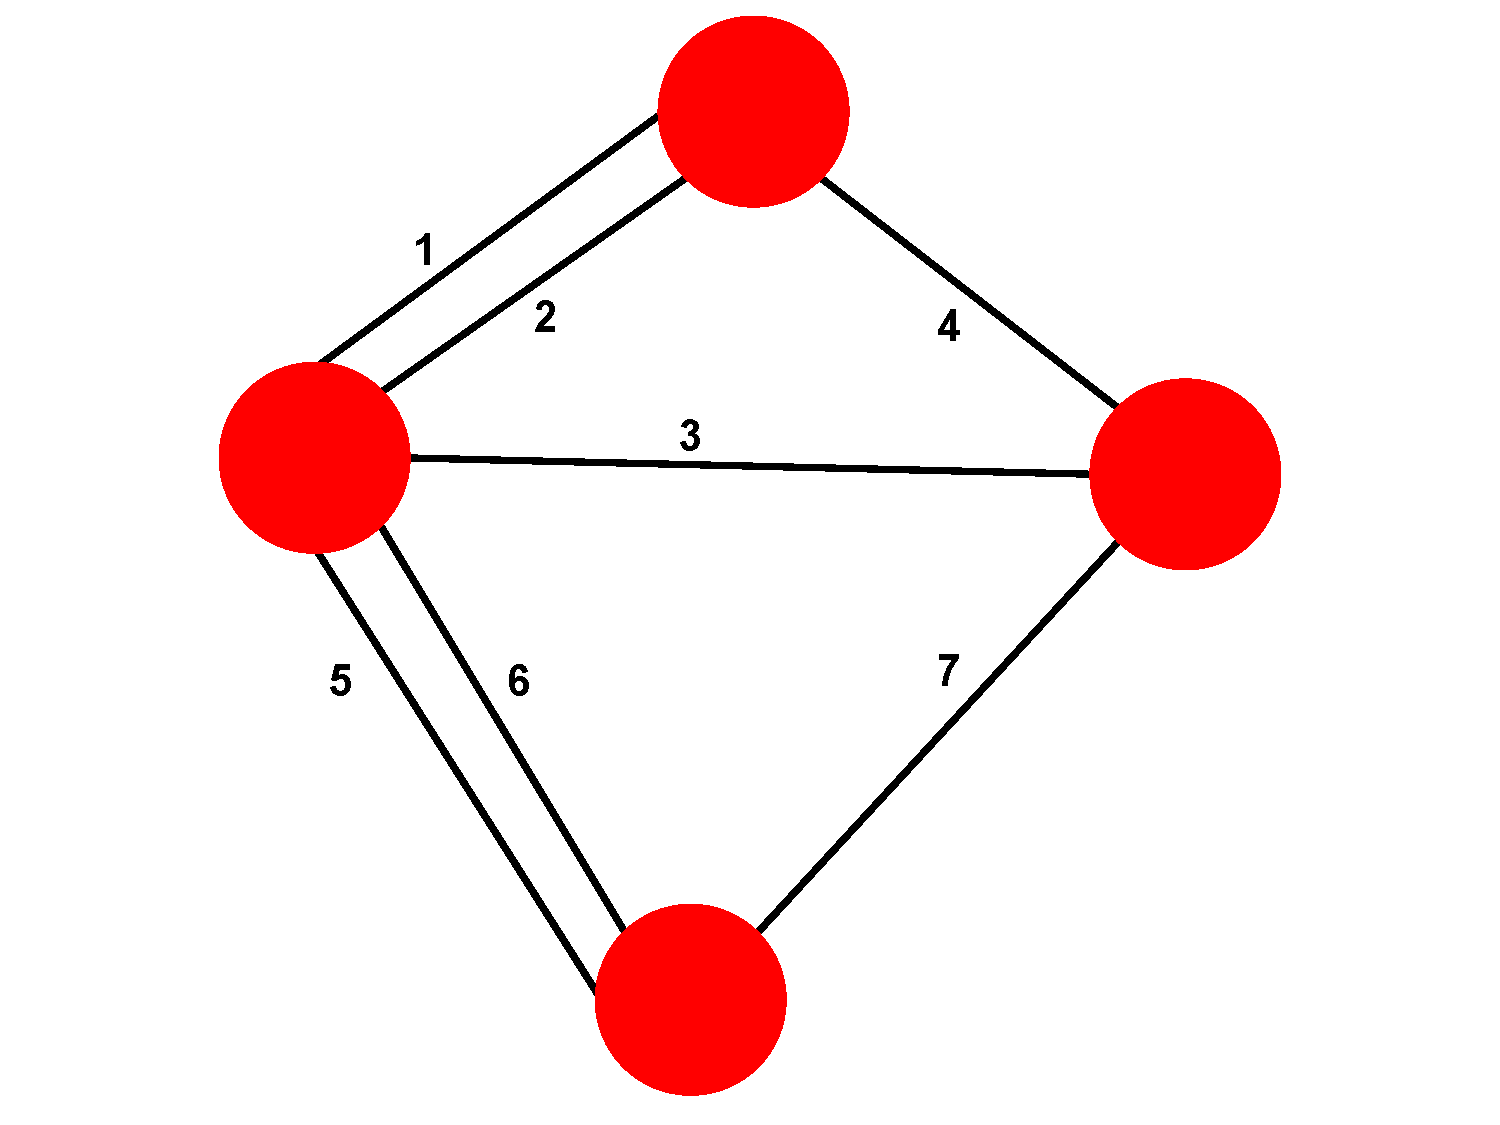
\includegraphics[width=.5\textwidth]{pictures/konigsberg.pdf}}}
    \caption{A graphical representation of the bridges of K\"{o}nigsberg.}\label{g_bridge}
\end{figure} 

The bridges of K\"{o}nigsberg is also a great example of how we can use graph theory to take information
from the real world and simplify it to make it easier to study. It is for this reason that Eulerian trails
have many practical uses. The most common use of them is likely navigation, especially for companies 
like mail carriers. These companies can look at roads as edges and houses as vertices, and they need
to visit every vertex as efficiently as possible. So they would find a closed Eulerian trail (if one
exists) beginning and terminating at their distribution center. Another use would be computer networking,
for similar reasons. You want to be able to connect computers and servers as efficiently as
possible. Closed Eulerian trails are also being used to help reconstruct DNA fragments. Eulerian trails
and graph theory are often really useful when it comes to studying how complex systems are connected.


\bibliographystyle{amsplain}
\begin{thebibliography}{10}

\bibitem{C} S. Carlson, K\"{o}nigsberg bridge problem: https://www.britannica.com/science/Konigsberg-bridge-problem

\bibitem{B} S. Belcastro, {\it Discrete Mathematics with Ducks}, CRC Press, 2012.

\bibitem{E} S. Epp, {\it Discrete Mathematics with Applications}, Brooks Cole, 1996.

\end{thebibliography}


\end{document}
